\newpage
\subsubsection{Simulering af kamera}
Til at generere et billedsæt, der simulerer langerhanske øer, er der udviklet et Matlab script. Scriptet består overordnet af 3 faser. Den første fase består i at segmentere langerhanske øer udfra et billede og oprette dem som en maske. I anden fase laves en maske bestående af ekstra væv, mens der i tredje fase simuleres flow. I den sidste fase gemmes også de enkelte billeder i formatet .png. De enkelte faser er nærmere beskrevet under deres afsnit. Der anvendes 3 billeder til grundlag for genereringen. Det ene billede viser isolerede øer. Det andet billede viser opløsningen indeholdende øer og ekstra væv. Det sidste billede er et baggrundsbillede uden øer eller ekstra væv. Dette billede anvendes som baggrund for de genererede billeder. Billederne der er valgt stammer fra det indkøbte kamera. Grunden til de kan anvendes som grundlag for genereringen af billeder, på trods af kameraets utilstrækkelige kvalitet, er at øerne og det ekstra væv er adskilt i de enkelte billeder. Dette muliggør en seperat segmentering af øer og væv, som  herefter kan sammensættes til billeder der ligger tæt op af det man observerer gennem et almindeligt mikroskop. De 3 billeder er vist herunder.

\begin{figure}[htbp] \centering
\begin{minipage}[b]{0.3\textwidth} \centering
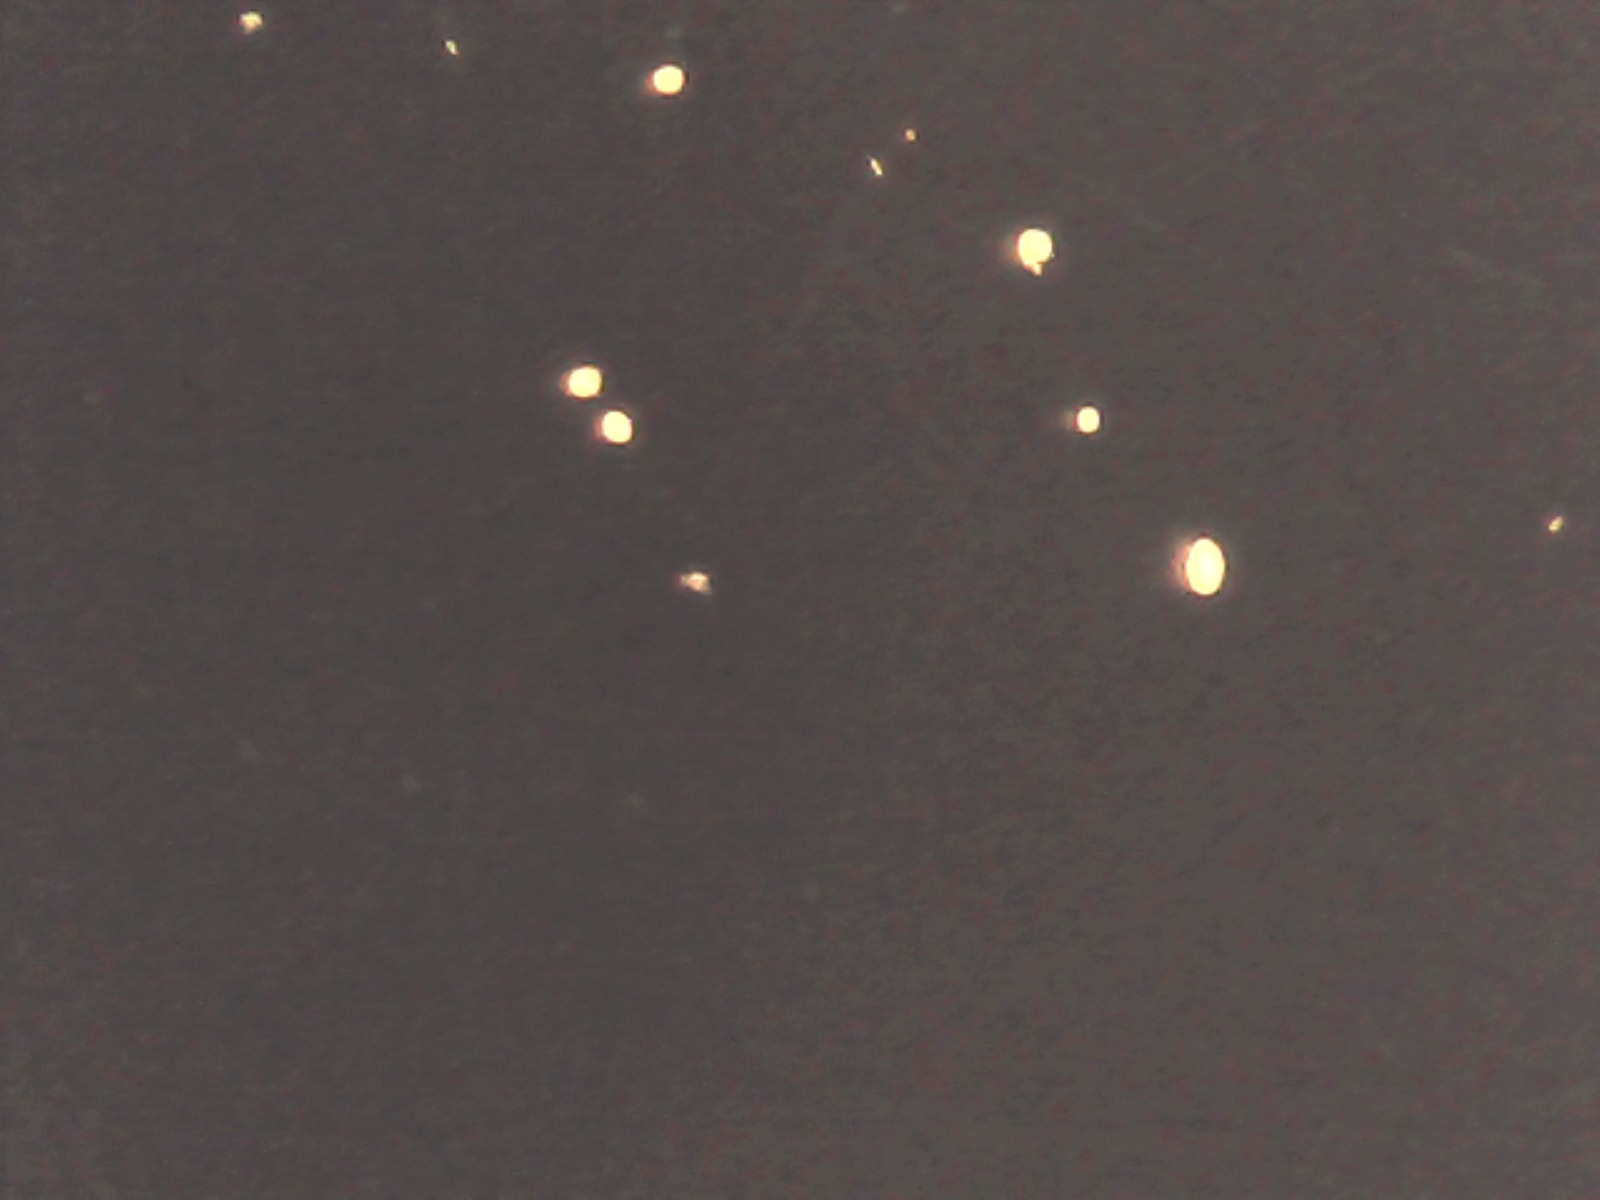
\includegraphics[width=1.00\textwidth]{billeder/software/1.jpg} % Left picture
\end{minipage} \hfill
\begin{minipage}[b]{0.3\textwidth} \centering
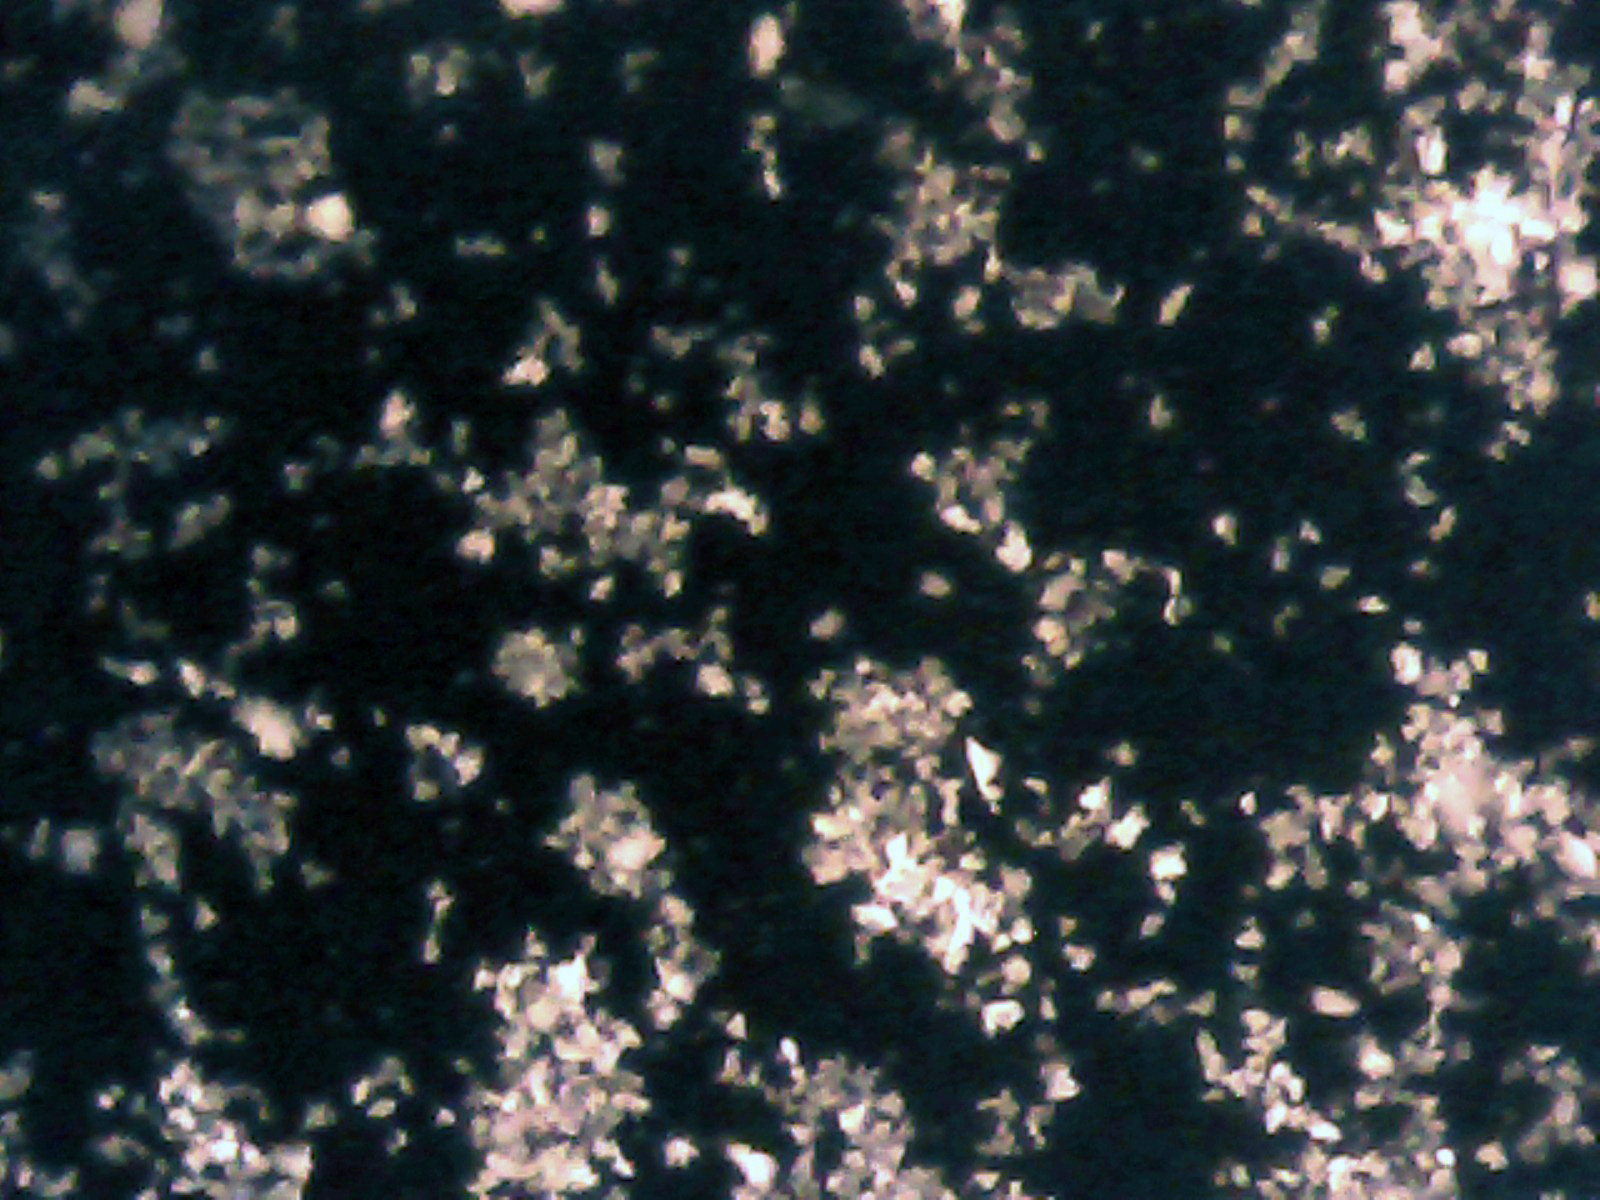
\includegraphics[width=1.00\textwidth]{billeder/software/2.jpg} % Right picture
\end{minipage} 
\hfill
\begin{minipage}[b]{0.3\textwidth} \centering

\includegraphics[width=1.00\textwidth]{billeder/software/3.jpg} % Right picture
\end{minipage} \\  % Captions og labels
\begin{minipage}[t]{0.3\textwidth}
\caption{Billede indeholdende langerhanske øer} % Left caption and label
\label{fig:img1}
\end{minipage} \hfill
\begin{minipage}[t]{0.3\textwidth}
\caption{Billede indeholdende ekstra væv} % Right caption and label
\label{fig:img2}
\end{minipage}
\hfill
\begin{minipage}[t]{0.3\textwidth}
\caption{Baggrundsbillede} % Right caption and label
\label{fig:img3}
\end{minipage}
\end{figure}

\textbf{Fase 1}

Segmenteringen af langerhanske øer sker ud fra billede 1 \ref{fig:img1}, hvor funktionen circleFinder anvendes til at finde centrum og radius på af de fundne celler. Resultatet af circlefinder segmenteringen er vist i fiugr \ref{fig:circlefinder}

 \begin{figure}[H]
	\centering
	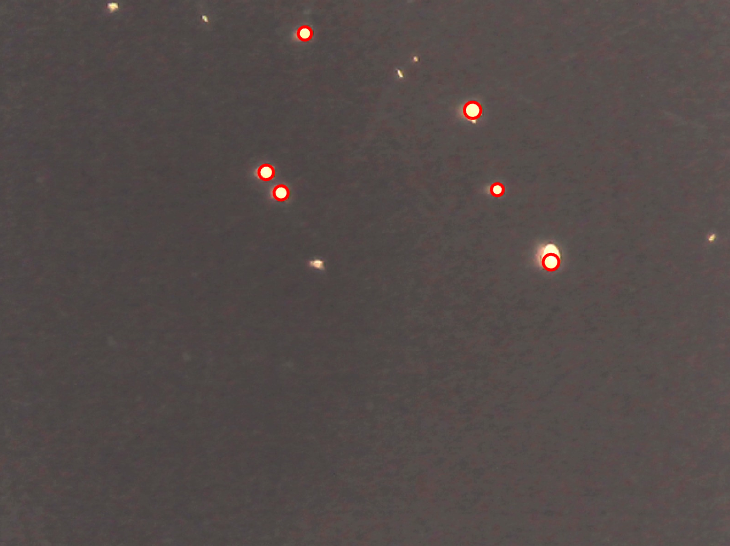
\includegraphics[width=0.5\textwidth]{billeder/software/circlefinder.png}
	\caption{Circlefinder til ø detektion}
	\label{fig:circlefinder}
\end{figure}

Circlefinder funktionen giver følgende funktion, som kan anvendes til at detektere cirkler med. Parametrene Sensitivty og edgeThreshold beskriver, hvor cirkulære objekterne er og generelt hvor følsom algoritmen er. Som det ses på figur \ref{fig:circlefinder} findes der kun én cirkel pr. ønsket ø.
\begin{lstlisting} 
detectCircles = @(x) imfindcircles(x,[12 30], ...
	'Sensitivity',0.8500, ...
	'EdgeThreshold',0.20, ...
	'Method','PhaseCode', ...
	'ObjectPolarity','Bright');
[centers, radii, metric] = detectCircles(im);
\end{lstlisting} 


\textbf{Fase 2}

I anden fase bliver det ekstra væv segmenteret ud fra billede 2 (figur \ref{fig:img2}). Til dette er der anvendt Color Threshold appen i Matlab. Ved hjælp af denne app er der lavet en funktion, som opretter en logisk maske af det ekstra væv. Opsætningen i appen er vist i figur (REF) \fxnote {Indsæt figur}. Yderligere er der anvendt morfologiske operationer til at fjerne uønskede objekter fra masken, samt fjerne støj. Til at fjerne uønskede objekter er funktionen \textit{bwareafilt} anvendt, med parametrene 150 og 500. Dette fjerner alle objekter under 150 og over 500 sammenhørende pixels. Til at udfylde huller i de enkelte objekter er funktionen \textit{imfill} brugt. 

\textbf{Fase 3}

I fase 3 sker selve flow simuleringen. Flowsimuleringen er opbygget på den måde, at den består af henholdvis en sekvens indeholdende en langerhansk ø efterfulgt af en sekvens uden en ø. I selve programmet indlæses et nyt billede hvert 0,1 sekund. Derfor skal der generes en passende mængde billeder, som programmet kan indlæse. Fase 3 er implementeret så der minimum genereres 252 eller maksimalt 432 billeder, hvilket giver en samlet sekvenslængde på 25,2 eller 43,2 sekund. Grunden til at antallet af billeder varierer er at længden af sekvensen uden en langerhansk ø bestemmes udfra en random variabel. Dette gøres for, at simulere at det kan være variabel tid mellem en ny ø kommer i gennem slangen. I scriptet genereres der i alt 18 fulde sekvenser. Det betyder, at der passerer i mellem 25 og 43 øer i minuttet. Antallet af øer der passere pr. minut er bestemt ud fra formel \ref{formular:isletprmin}: 
\begin{align}
\frac{18}{\frac{n}{10}} * 60 = \text{Antal øer pr. minut}
\text{ , hvor n er antallet af billeder i sættet}
\label{formular:isletprmin}
\end{align} 
I figur \ref{fig:boxplot} er vist et boxplot som viser distributionen af hvor mange øer der passere i minuttet. Det ses at medianen ligger over 30 øer pr. minut, hvilket betyder at der i gennemsnit vil komme over 30 øer pr minut. De 30 øer pr. minut stammer fra hastighedskravet fra systemets kvalitetskrav (\ref{subsec:qa}).

 \begin{figure}[H]
	\centering
	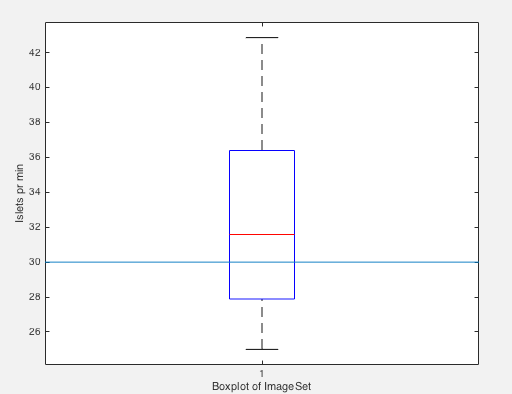
\includegraphics[width=0.5\textwidth]{billeder/software/boxplot.png}
	\caption{Boxplot af distrubutionen af øer pr. minut}
	\label{fig:boxplot}
\end{figure}

Selve flowsimuleringen sker i et for loop. Først udvælges en tilfældig celle ved hjælp af randi (uniform fordelt random variabel). I for loopet opdateres dens center position ud fra 2 variabler (newXPos og newYPos). X positionen springer med et fast interval for hver iteration (160 px). Inden for loopet fastsættes start positionen for cellen med \textit{randi}, som giver et tal mellem 0 og 1200 px (højden på billedet). Herefter opdateres den nye Y position ved hjælp af randn (normal fordelt random variabel) med middelværdi sat til startpositionen og en standard afvigelse på 50 pixels. I figur \ref{fig:flowsim} er flow simulationen illustreret for de i alt 18 sekvenser, med en graf for hver celle. Det ses at cellen flytter sin Y position tilfældigt, mens X positionen springer med et fast interval for hver iteration i for loopet.

\begin{figure}[H]
	\centering
	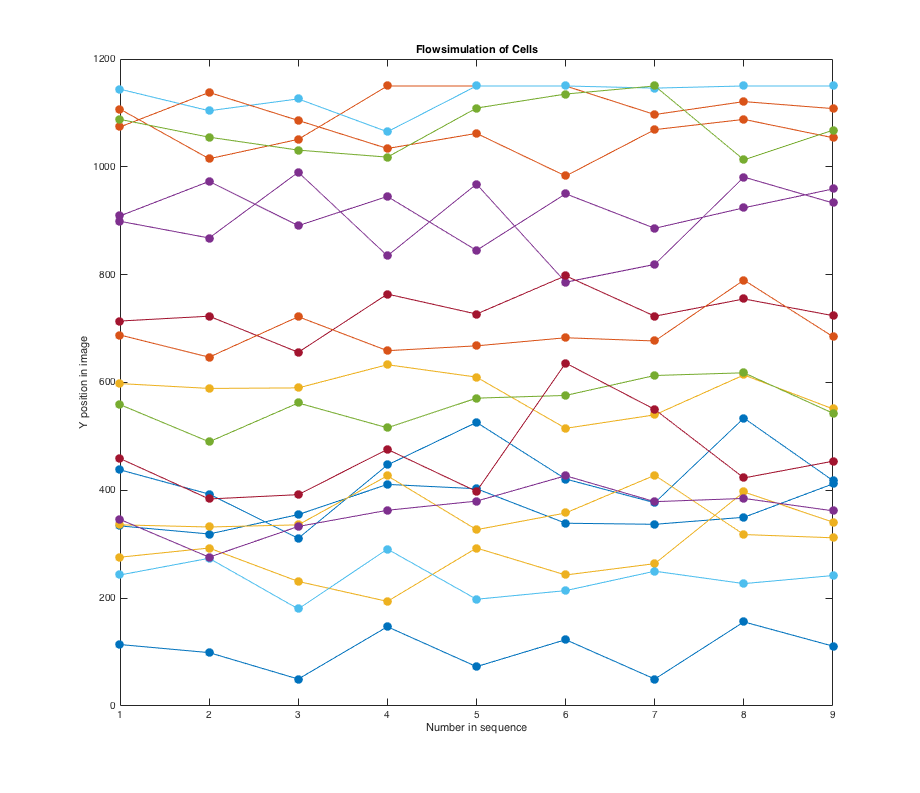
\includegraphics[width=0.5\textwidth]{billeder/software/Simulation.png}
	\caption{Illustration over flow simuleringen}
	\label{fig:flowsim}
\end{figure}

Efter generering af ny x og y position oprettes en maske for cellen ved brug af funktionen createCirclesMask. Til at indsætte cellen i baggrundsbilledet indekseres baggrundsbilledet med masken for cellen, så gråtoneværdierne fra det oprindelige billede indsættes.

Yderligere er der tilføjet tilfældig støj til billedet i form af “Salt and pepper” og gausisk hvid støj. Her er Matlab funktionen \textit{imnoise} anvendt. 

Masken med ekstra væv flyttes for hver iteration med funktionen \textit{circshift}, som bit shifter arrayet cirkulært. Parametrene definerer antallet af rækker og kolonner arrayet skal shiftes.  Antallet af kolonner er fastdefineret til 160 px, mens rækkerne skiftes efter en normalfordelt random variabel med mean på 0 og standard afvigelse på 50 pixels. Nedenstående figur \ref{fig:histfit} viser fordelingen af antallet af rækker der flyttes. På figur \ref{fig:histfit} er der vist markører for standard afvigelsen ($\sigma$) og $2*$standard afvigelsen ($2\sigma$) for hver side af mean. I mellem $-\sigma$ og $\sigma$ er der 68,26 \% sandsynlighed for, at den nye Y position ville ligge inden for dette område. For 2 sd afvigelse ($2\sigma$) er der 95,45 \% for, at den nye Y position vil ligge inden for dette område.

\begin{figure}[H]
	\centering
	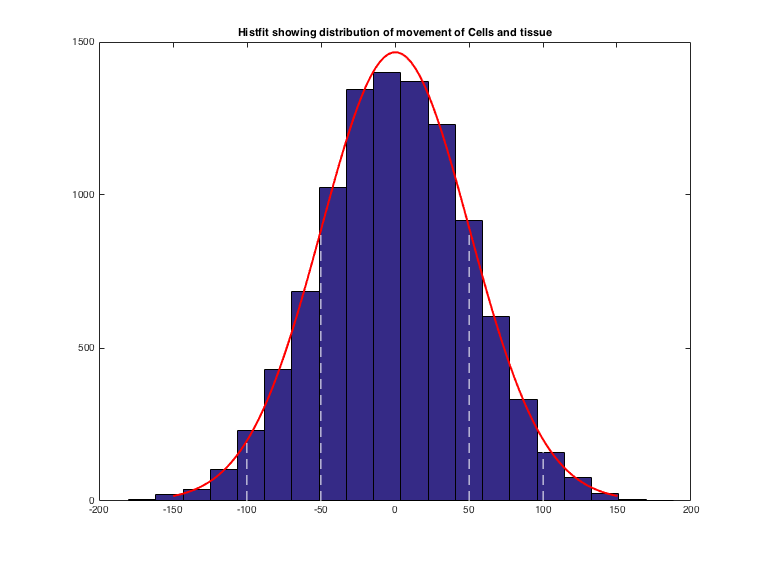
\includegraphics[width=0.5\textwidth]{billeder/software/histfit.png}
	\caption{Histogram over fordelingen af ny Y position}
	\label{fig:histfit}
\end{figure}

Det endelige resultat af billedegeneringen er vist i figur \ref{fig:finalresult}. Til at illustrere hvordan øen flytter sig er der tilføjet en graf, som viser hvordan dens position ændres for hver iteration. Cellen er markeret med en rød ring på billedet.

\begin{figure}[H]
	\centering
	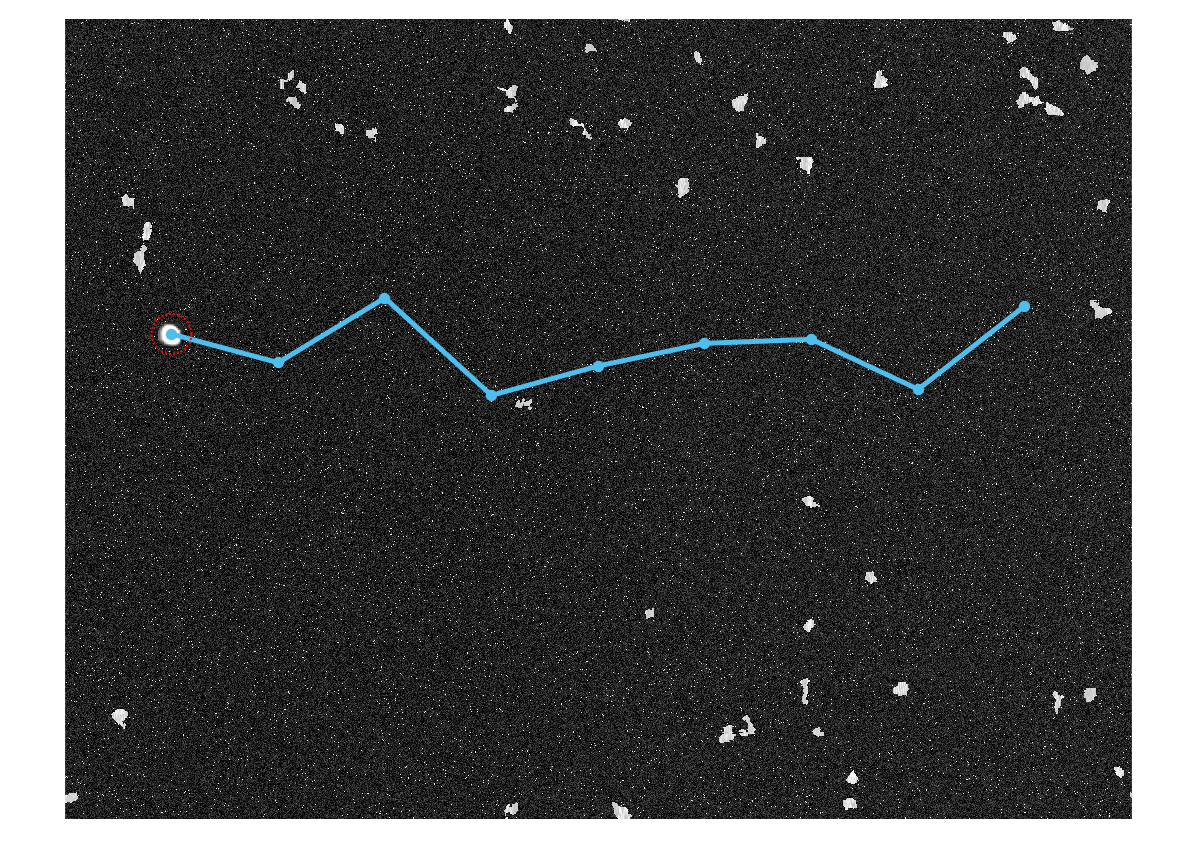
\includegraphics[width=0.7\textwidth]{billeder/software/final.png}
	\caption{Endelige resultat for flowsimulering}
	\label{fig:finalresult}
\end{figure}

Implementeringen af scriptet er vedlagt i bilag \fxnote{Indsæt referencer til bilag}